\section{并行与并发}
Rust也同样支持常见的并行和并发操作,也同样分为进程,线程以及消息通信等等。

\subsection{线程}
Rust的线程操作必须使用闭包完成。在之前看到的闭包当中,通常采用的都是有参的闭包,
而在Rust的线程操作当中,则经常会遇到无参数的闭包;Rust的线程使用thread::spawn函数
进行实现:
\begin{code-block}{rust}
use std::thread;
use std::time::Duration;

fn main() {
    thread::spawn(|| {
        for i in 1..10 {
            println!("hi number {} from the spawned thread!", i);
            thread::sleep(Duration::from_millis(1));
        }
    });

    for i in 1..5 {
        println!("hi number {} from the main thread!", i);
        thread::sleep(Duration::from_millis(1));
    }
}
\end{code-block}
和其他语言的线程概念一样,当主线程结束时,所有的线程都会被终止。因此上述代码当中,
子线程(spawn)无法将所有的循环执行完成。为了达成所有进/线程执行完成之后才退出主
进/线程的目的,和其他的开发语言相同,需要在主进程当中调用join函数:
\begin{code-block}{rust}
fn main() {
    let handle = thread::spawn(|| {
        for i in 1..10 {
            println!("hi number {} from the spawned thread!", i);
            thread::sleep(Duration::from_millis(1));
        }
    });

    for i in 1..5 {
        println!("hi number {} from the main thread!", i);
        thread::sleep(Duration::from_millis(1));
    }
    handle.join().unwrap();
}
\end{code-block}
Thread::spawn的返回值是JoinHandle,是一个拥有所有权的值,当对其调用join方法时,
它会等待对应线程结束;而join的返回值是一个Result,可以按照之前介绍的方式进行处理。
同时,Join函数是一个阻塞式函数,只有当该函数运行结束之后,才会继续进行后续的操作。

多数情况下,Rust的线程不可能只会在内部运行,而和外部没有数据交互。但是,如果我们
直接使用外部数据,则会出现错误,比如下方的代码:
\begin{code-block}{rust}
fn main() {
    let v = vec![1, 2, 3];
    let handle = thread::spawn(|| {
        println!("Here's a vector: {:?}", v);
    });
    handle.join().unwrap();
}
\end{code-block}
\begin{figure}[H]
  \centering
  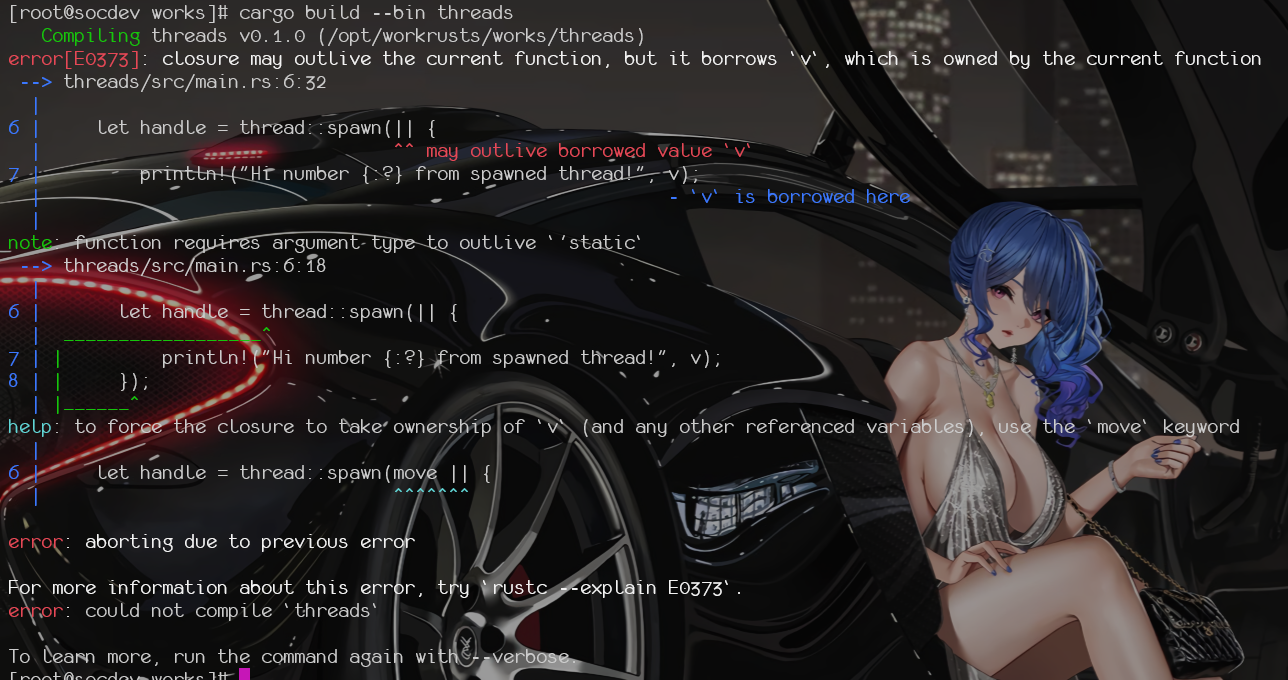
\includegraphics[width=\linewidth]{rust_thread_out_params.png}
  \caption{试图访问线程外部资源}
  \label{fig:rust_thread_out_params}
\end{figure}
线程使用的是闭包,从闭包的定义来说,是可以捕获并使用外部变量和数据的;但是,Rust
不知道这个线程到底会运行多长时间,因此无法知道对外部变量的引用是否一直有效,比如
下方的代码:
\begin{code-block}{rust}
fn main() {
    let v = vec![1, 2, 3];
    let handle = thread::spawn(|| {
        println!("Here's a vector: {:?}", v);
    });
    drop(v);
    handle.join().unwrap();
}
\end{code-block}
启动线程的同时,立即将v进行丢弃,线程内部无法知道v在运行阶段是否继续有效,就会
出现错误,因此,如果在线程当中使用默认的闭包模式,则无法对应的闭包是无法捕获以及
使用外部的变量和数据的。此时,则需要使用move闭包进行替换,即强制闭包获取外部变量
的所有权,而不是由Rust进行借用推断。但是需要注意,一旦使用move之后,在线程之外,
变量将无法再进行使用:
\begin{code-block}{rust}
fn main() {
    let v = vec![1, 2, 3];
    let handle = thread::spawn(move || {
        println!("Here's a vector: {:?}", v);
    });
    // 下方代码无法再进行执行
    // println!("{:?}", v);
    handle.join().unwrap();
}
\end{code-block}

\subsection{消息通信和消息传递}
每个线程做自己的事情,但是,不管什么编程语言,都需要考虑线程之间的数据交互问题。
Rust向Golang进行了学习,使用通信替换共享内存,来进行线程之间的数据传输。同样的,
Rust当中用于消息传递并发的主要工具是通道,该概念和Golang的通道概念相同。Rust的通道
分为2个角色:发送者和接收者,发送者发送消息,接收者接收消息,当发送者或者接收者任一
被丢弃时,则对应的通道被视为关闭。

Rust的通道采用mpsc::channel函数实现,mpsc表示多个生产者,单个消费者,因此,Rust
标准库实现通道的方式意味着一个通道可以有多个产生值的发送(sending)端,但只能有
一个消费这些值的接收(receiving)端。通道的实现示例如下:
\begin{code-block}{rust}
use std::sync::mpsc;
fn main() {
    let (sender, recevier) = mpsc::channel();
}
\end{code-block}
其中,函数的第一个返回值为发送者,第二个参数为接收者。使用通道发送数据通信的示例
如下:
\begin{code-block}{rust}
use std::sync::mpsc;
use std::thread;

fn main() {
    let (sender, recevier) = mpsc::channel();

    thread::spawn(move || {
        let val = "lucifer".to_string();
        match sender.send(val) {
            Ok(_) => println!("Send success"),
            Err(error) => println!("Send failed :{:?}", error),
        }
    });

    let res = match recevier.recv() {
        Ok(s) => s,
        Err(error) => {
            println!("Cannot recevie anything from sender: {:?}", error);
            "".to_string()
        }
    };
    println!("The result of channel is {}", res);
}
\end{code-block}
接收者接收消息有2种模式:默认的recv是阻塞式,返回一个Result<T, E>,当通道关闭时,
将返回Result当中的Error;而try\_recv是非阻塞式,同样是返回一个Result<T, E>,但是,
Result当中的Error表示没有接收到任何消息,可以使用for循环进行反复的尝试读取操作。
另外需要注意的是,Send函数会改变变量的所有权,当该函数执行之后,被发送的消息
(变量)将无法再使用。

但是,通道可以反复使用,而且和Golang的类似,Rust的通道也是可以进行迭代的,特别
是在接收消息时,通常采用for循环进行操作,减少了错误处理的代码,使得代码更具可读性:
\begin{code-block}{rust}
use std::sync::mpsc;
use std::thread;

fn main() {
    let (sender, recevier) = mpsc::channel();

    let handler = thread::spawn(move || {
        let vals = vec!["lucifer", "titans", "garuda"];
        for val in vals {
            match sender.send(val) {
                Ok(_) => println!("Send success"),
                Err(error) => println!("Send failed :{:?}", error),
            }
        }
    });

    for msg in recevier {
        println!("The msg is {}", msg);
    }

    match handler.join() {
        Err(error) => println!("Error{:?}", error),
        _ => (),
    }
}
\end{code-block}

同样的,由于Rust的通道默认是多生产者/单消费者,因此,可以通过多个发送端向单个接
收端发送消息。实际使用当中的多个发送端,则通常是某个发送端的克隆对象,如下:
\begin{code-block}{rust}
use std::sync::mpsc;
use std::thread;

fn main() {
    let (sender, recevier) = mpsc::channel();
    let sender_copy = sender.clone();

    let handler = thread::spawn(move || {
        let vals = vec!["lucifer", "titans", "garuda"];
        for val in vals {
            match sender.send(val) {
                Ok(_) => println!("Send success"),
                Err(error) => println!("Send failed :{:?}", error),
            }
        }
    });

    let handler_copy = thread::spawn(move || {
        let vals = vec!["zhangjl", "luoyan", "zhangzz"];
        for val in vals {
            match sender_copy.send(val) {
                Err(error) => println!("Send failed :{:?}", error),
                _ => (),
            }
        }
    });

    for msg in recevier {
        println!("The msg is {}", msg);
    }

    match handler_copy.join() {
        Err(error) => println!("Error{:?}", error),
        _ => (),
    }

    match handler.join() {
        Err(error) => println!("Error{:?}", error),
        _ => (),
    }
}
\end{code-block}

\subsection{共享状态}
在其他语言当中,有些特殊的场景,还是必须使用原有的线程并发概念——锁——来进行资源的
访问/读写控制。Rust当中同样存在锁,比较常见的就是互斥锁(互斥器,Mutex)以及原子
计数器(Arc)。在基本的操作上,互斥锁的使用和其他语言当中没有太大的区别:
\begin{code-block}{rust}
use std::sync::Mutex;
fn main() {
    let m = Mutex::new(5);
    {
        let mut num = m.lock().unwrap();
        *num = 6;
    }
    println!("m = {:?}", m);
}
\end{code-block}
注意,上述代码如果将内部大括号去除,则运行结束之后,m的状态还是锁定状态;但是,
有大括号,则表示大括号内部的段是一个有效的生命周期,当该生命周期结束之后,互斥
锁将自动释放。一旦获取了锁,就可以将返回值(在这里是num)视为一个其内部数据的
\underline{\color{red} \textbf{可变引用}}。类型系统确保了我们在使用m中的值之前
获取锁:Mutex<i32>并不是一个i32,所以必须获取锁才能使用这个i32值。

实质上,Mutex是一个智能指针,lock调用返回一个叫做MutexGuard的智能指针。这个智能
指针实现了Deref来指向其内部数据;同时也提供了一个Drop实现,使得MutexGuard离开作
用域时自动释放锁,即锁的释放是自动发生的。

但是默认情况下,Mutex是无法用于进行线程间的数据共享,如下:
\begin{code-block}{rust}
use std::rc::Rc;
use std::sync::Mutex;
use std::thread;

fn main() {
    let counter = Rc::new(Mutex::new(0));
    let mut handles = vec![];

    for _ in 0..10 {
        let counter = Rc::clone(&counter);
        let handle = thread::spawn(move || {
            let mut num = counter.lock().unwrap();

            *num += 1;
        });
        handles.push(handle);
    }

    for handle in handles {
        handle.join().unwrap();
    }

    println!("Result: {}", *counter.lock().unwrap());
}
\end{code-block}
上述代码会出现下面的类似错误:
\begin{figure}[H]
  \centering
  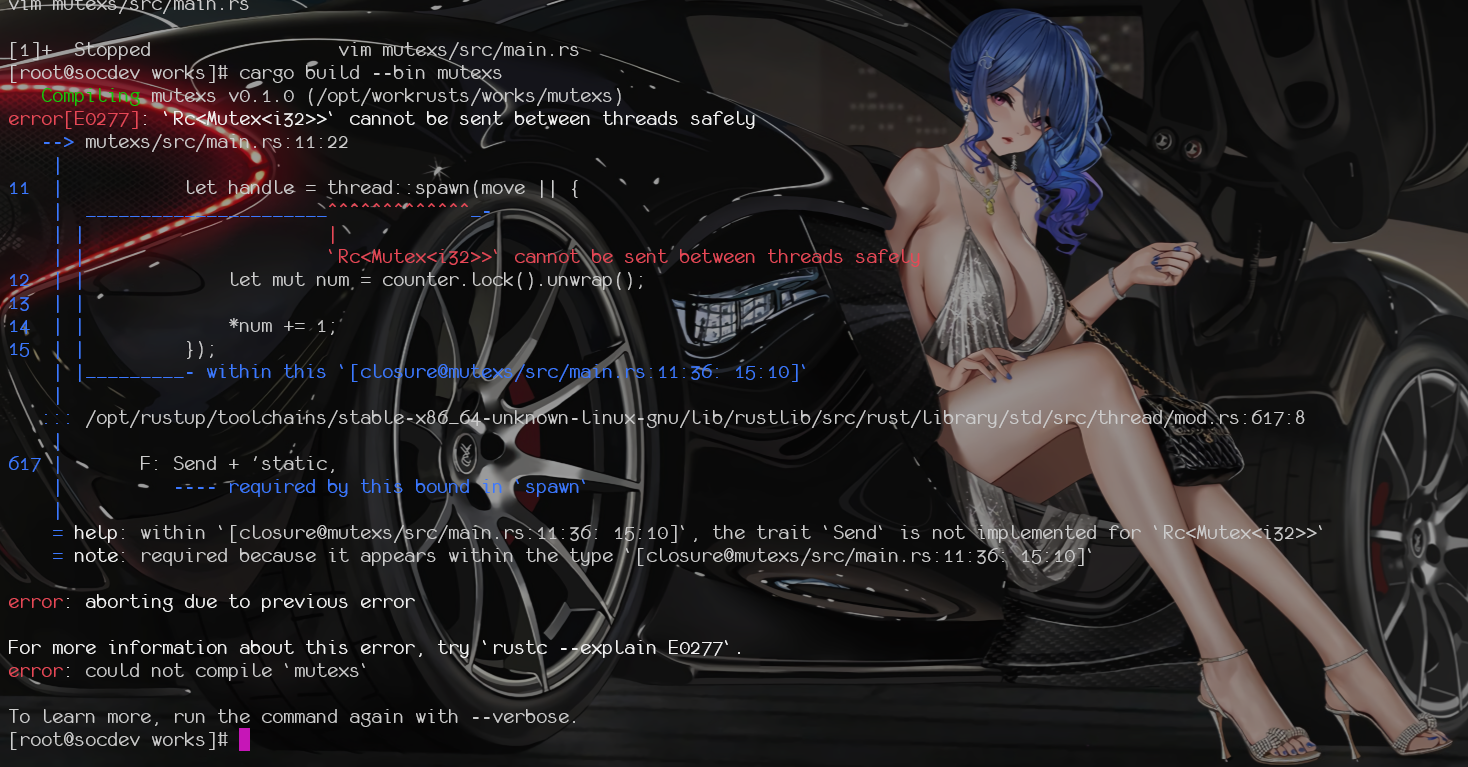
\includegraphics[scale=0.215]{rust_mutex_share_error.png}
  \caption{试图通过Rc共享Mutex的数据}
  \label{fig:rust_mutex_share_error}
\end{figure}
即之前提到的,Rc类型只能用于单线程/单进程环境。

而共享引用计数则需要使用Arc,它是可以安全的用于并发环境的类型,即原子引用计数,
可以在线程间进行共享所有权。Arc和Rc有相同的API,基本使用方法上类似。所有,可以直
接对上述代码进行修改:
\begin{code-block}{rust}
use std::sync::{Arc, Mutex};
use std::thread;
fn main() {
    let counter = Arc::new(Mutex::new(0));
    let mut handles = vec![];
    for _ in 0..10 {
        let counter = Arc::clone(&counter);
        let handle = thread::spawn(move || {
            let mut num = counter.lock().unwrap();
            *num += 1;
        });
        handles.push(handle);
    }
    for handle in handles {
        handle.join().unwrap();
    }
    println!("Result: {}", *counter.lock().unwrap());
}
\end{code-block}
通过这样简单的修改,成功实现了10个进程当中对同一个数值进行加法操作的功能。

\section{Match与模式匹配}
Match是Rust常用的语法糖,其用法不局限于之前所讲的范围。关于match的用法,还有很多,
并且,多数和模式匹配有关,接下来可以看一些常见的match和模式匹配的使用方式。
\begin{outline}[enumerate]
\1 多种匹配模式

在match表达式当中,可以用|匹配多个模式,表示或运算:
\begin{code-in-enumerate}{rust}
let x = 1;
match x {
    1 | 2 => println!("one or two"),
    3 => println!("three"),
    _ => println!("anything"),
}
\end{code-in-enumerate}

\1 使用..=匹配范围

..=语法允许匹配一个数值范围内的任意数据,常用于数值和字符:
\begin{code-in-enumerate}{rust}
let x = 5;
match x {
    1..=5 => println!("one through five"),
    _ => println!("something else"),
}

let y = 'c';
match y {
    'a'..='j' => println!("early ASCII letter"),
    'k'..='z' => println!("late ASCII letter"),
    _ => println!("something else"),
}
\end{code-in-enumerate}

\1 解构结构体

Let模式可以将结构体当中的字段/元素进行解构,单独或者批量赋予其他元素:
\begin{code-in-enumerate}{rust}
struct Point {
    x: i32,
    y: i32,
}
fn main() {
    let p = Point { x: 0, y: 7 };
    // 将p的x字段的值赋予a,y字段的值赋予b,a和b是整数类型,不是引用
    let Point { x: a, y: b } = p;
    // let Point {x: ref a, y: ref b} = p; 和上面类似,但是a和b是整数类型的引用
    // let Point {x: a, y: _} = p; 表示只需要将x的值赋予a,但不需要对y进行解构
    assert_eq!(0, a);
    assert_eq!(7, b);
    // let Point {x, y} = p; 将p的x字段的值赋予变量x,y字段的值赋予变量y
}
\end{code-in-enumerate}

\1 解构枚举类型

Match本身就是应枚举而生的,因此天然的可以使用它对枚举进行解构:
\begin{code-in-enumerate}{rust}
enum Message {
    Quit,
    Move { x: i32, y: i32 },
    Write(String),
    ChangeColor(i32, i32, i32),
}

fn main() {
    let msg = Message::ChangeColor(0, 160, 255);

    match msg {
        Message::Quit => {
            println!("The Quit variant has no data to destructure.")
        }
        Message::Move { x, y } => {
            println!("Move in the x direction {} and in the y direction {}", x, y);
        }
        Message::Write(text) => println!("Text message: {}", text),
        Message::ChangeColor(r, g, b) => {
            println!("Change the color to red {}, green {}, and blue {}", r, g, b)
        }
    }
}
\end{code-in-enumerate}

同样的,如果枚举当中嵌套了枚举,仍然可以使用match进行解构:
\begin{code-in-enumerate}{rust}
enum Color {
    Rgb(i32, i32, i32),
    Hsv(i32, i32, i32),
}

enum Message {
    Quit,
    Move { x: i32, y: i32 },
    Write(String),
    ChangeColor(Color),
}

fn main() {
    let msg = Message::ChangeColor(Color::Hsv(0, 160, 255));

    match msg {
        Message::ChangeColor(Color::Rgb(r, g, b)) => {
            println!("Change the color to red {}, green {}, and blue {}", r, g, b)
        }
        Message::ChangeColor(Color::Hsv(h, s, v)) => {
            println!(
                "Change the color to hue {}, saturation {}, and value {}",
                h, s, v
            )
        }
        _ => (),
    }
}
\end{code-in-enumerate}

\1 解构复合数据

用复杂的方式来混合、匹配和嵌套解构模式,解析出我们感兴趣的数据:
\begin{code-in-enumerate}{rust}
let ((feet, inches), Point {x, y}) = ((3, 10), Point { x: 3, y: -10 });
\end{code-in-enumerate}

\1 忽略不需要的元素

在Rust的当中,默认可以使用\_对不必要的变量进行忽略,通常用在match的最后分支,但是,
实际上也可以用去其他任意的模式,甚至是函数参数:
\begin{code-in-enumerate}{rust}
// 需要传入2个参数,但是忽略第一个参数
fn foo(_: i32, y: i32) {
    println!("This code only uses the y parameter: {}", y);
}

fn main() {
    foo(3, 4);
}
\end{code-in-enumerate}

除了使用\_进行忽略之外,还可以使用..语法糖进行忽略,但是针对结构体和元组存在区别:
结构体当中,忽略的是没有被列出的字段;而元组忽略的则是范围:
\begin{code-in-enumerate}{rust}
struct Point {
    x: i32,
    y: i32,
    z: i32,
}

fn main() {
    let origin = Point { x: 0, y: 0, z: 0 };
    // 将point的y进行忽略
    match origin {
        Point { x,z, .. } => println!("x is {}, z is {}", x, z),
    }

    let numbers = (2, 4, 8, 16, 32);
    match numbers {
        // 忽略元组当中除第1、2和最后一项的所有元素
        (first, second, .., last) => {
            println!("Some numbers: {}, {}, {}, ", first, second, last);
        }
    }
}
\end{code-in-enumerate}

同样的,忽略操作也可以用于闭包当中:
\begin{code-in-enumerate}{rust}
let player_scores = [("Jack", 20), ("Jane", 23), ("Jill", 18), ("John", 19)];
// 对player_scores进行迭代,忽略其中第二个元素,_可以被替换为_score
let players: Vec<_> = player_scores.iter().map(|&(player, _)| player).collect();
// 输出的结果当中将只会有字符串数据
println!("{:?}", players);
\end{code-in-enumerate}


\1 @绑定

运算符@允许我们在创建一个存放值的变量的同时测试其值是否匹配模式,比如测试字段是
否位于指定范围内,同时也希望能将其值绑定到另外的变量中以便此分支相关联的代码可以
使用它:
\begin{code-in-enumerate}{rust}
enum Message {
    Hello { id: i32 },
}

let msg = Message::Hello { id: 5 };

match msg {
    // 将变量id保存到另一个变量ip_variable当中
    Message::Hello { id: id_variable @ 3..=7 } => {
        println!("Found an id in range: {}", id_variable)
    },
    Message::Hello { id: 10..=12 } => {
        println!("Found an id in another range")
    },
    Message::Hello { id } => {
        println!("Found some other id: {}", id)
    },
}
\end{code-in-enumerate}
\end{outline}

\section{高级特征}
Rust设计不仅仅是为了开发应用程序,其设计之初,就是为了解决内存安全的问题,并且可以
广泛用于各种场景,包括C语言的专属领域:操作系统设计。在编写操作系统的过程当中,
C语言使用了很多的高级宏定义以及一些精妙的设计,而Rust同样如此。为了和硬件打交道,
Rust被设计为可以拥有直接操作硬件的能力,这些都是其高级特性的一部分。Rust的高级
特性主要包含下列内容:
\begin{enumerate}
  \item 不安全 Rust
  \item 高级 Trait
  \item 高级函数和闭包
  \item 宏
\end{enumerate}

\subsection{Unsafe}
Rust屏蔽了一系列的不安全操作来换取应用程序的稳定性和可靠性,但是,可以通过关键字
unsafe,切换到不安全的运行环境当中,并且在unsafe的代码块当中运行。常见的不安全操作
如下:
\begin{enumerate}
  \item 解引用裸指针
  \item 使用不安全的方法/函数
  \item 访问/修改可变的静态变量
  \item 实现不安全的Trait
  \item 访问union的字段
\end{enumerate}
在使用的时候,原则需要明确:保持unsafe块尽可能小,将不安全代码封装进一个安全的
抽象并提供安全API是一种常见的安全操作和手段。

所谓的裸指针,和普通的指针和智能指针相比,存在如下的区别:
\begin{enumerate}
  \item 允许忽略借用规则,可以同时拥有不可变和可变的指针,或多个指向相同位置的可变指针
  \item 不保证指向有效的内存
  \item 允许为空
  \item 不能实现任何自动清理功能
\end{enumerate}
Rust当中存在2个裸指针:分别写作*const T(不可变)和*mut T(可变),其基本的定义方式
如下:
\begin{code-block}{rust}
let mut num = 5;
let r1 = &num as *const i32; // 不可变的裸指针
let r2 = &mut num as *mut i32; // 可变的裸指针
\end{code-block}

裸指针的定义是安全的,但是,它的使用是不安全的,因此裸指针的使用必须在unsafe块
当中:
\begin{code-block}{rust}
fn main() {
    let mut num = 5;

    let r1 = &num as *const i32;
    let r2 = &mut num as *mut i32;

    unsafe {
        *r2 = 10;
        // r1,r2和num都会变更为10
        println!("{},{}", *r1, *r2);
    }
}
\end{code-block}
同样的,unsafe也可以用于定义函数/方法,不过也需要在unsafe块当中使用;但是,unsafe
的方法可以作为安全方法进行导出,在使用时,则不需要使用unsafe进行标记:
\begin{code-block}{rust}
fn main() {
    let mut num = 5;
    // 定义裸指针
    let r1 = &num as *const i32;
    let r2 = &mut num as *mut i32;

    // 使用不安全的函数/方法
    unsafe {
        unsafe_change(r1, r2);
    }
    println!("{}", num);

    safe_change(r1, r2);
    println!("{}", num);
}

// 定义不安全的函数/方法
unsafe fn unsafe_change(r1: *const i32, r2: *mut i32) {
    *r2 = 10;
    println!("{},{}", *r1, *r2);
}

// 将不安全的函数/方法封装进安全的方法当中
fn safe_change(r1: *const i32, r2: *mut i32) {
    unsafe {
        *r2 = 100;
    }
}
\end{code-block}

作为不安全的一部分,某些时候直接在Rust当中调用C语言的类库可以获得更好的性能,此时,
则同样需要在unsafe块当中使用,比如在Rust当中调用标准C的abs(绝对值)函数:
\begin{code-block}{rust}
extern "C" {
    fn abs(input: i32) -> i32;
}

fn main() {
    unsafe {
        println!("The unsafe from C: {}", abs(-200));
    }
}
\end{code-block}
上述代码出现的extern关键字,有助于创建和使用外部函数接口(Foreign Function
Interface,FFI)。外部函数接口是一个编程语言用以定义函数的方式,其允许不同(外部)
编程语言调用这些函数。Extern块中声明的函数在Rust代码中总是不安全的,

特别需要注意的是,Rust当中的可变全局变量(static)同样是不安全的,需要在unsafe
代码块当中使用;而不可变的全局常量(const和static)则不需要在unsafe块当中;另外,
全局变量同样可以是任意数据类型的:
\begin{code-block}{rust}
use std::fmt;

struct Version {
    major: u8,
    minor: u8,
}

impl fmt::Display for Version {
    fn fmt(&self, f: &mut fmt::Formatter) -> fmt::Result {
        write!(
            f,
            "The version of this bin is {}.{}",
            self.major, self.minor
        )
    }
}

// 不可变的全局常量
const __CONST_NUM__: Version = Version { major: 1, minor: 4 };
const __VERSION__: &str = "v1.4.0";
static __NAME__: &str = "lucifer";
// 可变的全局变量
static mut __COUNTER__: u8 = 1;

fn main() {
    println!("{}", __CONST_NUM__);
    println!("{}", __NAME__);
    unsafe {
        println!("{}", __COUNTER__);
    }
}
\end{code-block}

\subsection{高级Trait}
Trait的语法当中,使用了如下的代码形式:
\begin{code-block}{rust}
impl Iterator for Counter {
    type Item = u32;
    fn next(&mut self) -> Option<Self::Item> {
        ...
    }
}
\end{code-block}
其中,type Item表示关联数据类型,Item表示占位类型,next方法定义表明它返回
Option<Self::Item>类型的值。这个trait的实现者会指定Item的具体类型。

在Trait当中,除了默认方法,方法覆写之外,还存在着运算符重载的功能。但是,和C++
不同,Rust并不允许创建自定义的运算符,或者重载任意运算符,只有std::ops当中所列出
的运算符和相应的trait可以通过实现运算符相关的trait来实现重载,比如下面,实现Add
trait来实现对+的运算符重载:
\begin{code-block}{rust}
use std::fmt;
use std::ops::{Add, AddAssign};

struct Point {
    x: u8,
    y: u8,
}

// 实现结构体的 c = a + b
impl Add for Point {
    type Output = Point;
    fn add(self, other: Point) -> Point {
        Point {
            x: self.x + other.x,
            y: self.y + other.y,
        }
    }
}

// 实现结构体的 a = a + b;
impl AddAssign for Point {
    fn add_assign(&mut self, other: Point) {
        self.x = self.x + other.x;
        self.y = self.y + other.y;
    }
}

impl fmt::Display for Point {
    fn fmt(&self, f: &mut fmt::Formatter) -> fmt::Result {
        write!(f, "x:{}, y:{}", self.x, self.y)
    }
}

fn main() {
    let a = Point { x: 3, y: 4 };
    let b = Point { x: 5, y: 6 };
    let c = a + b;

    let mut d = Point { x: 100, y: 101 };
    d = d + c;
    println!("{}", d);
}
\end{code-block}

以Add Trait为例,其内部的实现如下:
\begin{code-block}{rust}
#[lang = "add"]
pub trait Add<Rhs = Self> {
    type Output;
    #[must_use]
    fn add(self, rhs: Rhs) -> Self::Output;
}
\end{code-block}
其中,RHS=Self这个语法叫做默认类型参数。RHS是一个泛型类型参数,它用于定义add方法
中的rhs参数。如果实现Add trait时不指定RHS的具体类型,RHS的类型将是默认的Self类型
也就是在实现Add Trait的类型。在上述例子当中,RHS就是Point这个类型。但是,也可以使用
不同的数据类型,比如下面的例子:
\begin{code-block}{rust}
struct Meters(i32);
struct Millimeters(i32);

impl Add<Meters> for Millimeters {
    type Output = Millimeters;

    fn add(self, other: Meters) -> Millimeters {
        Millimeters(self.0 + (other.0 * 1000))
    }
}
\end{code-block}
定义一个结构体米,和结构体毫米,然后定义毫米与米的加法操作,当结构体毫米与结构体
米进行相加时(注意顺序),将结果转换成毫米结果:
\begin{code-block}{rust}
let meters = Meters(1);
let mill_meters = Millimeters(10);
let mill_meters_other = mill_meters + meters;
\end{code-block}
但是,如果将上述代码的顺序更换如下:
\begin{code-block}{rust}
let mill_meters_other = meters + mill_meters;
\end{code-block}
则会出现如下的错误:
\begin{figure}[H]
  \centering
  
\includegraphics[width=\linewidth]{rust_override_error.png}
  \caption{尝试进行不同类型的加法重载操作}
  \label{fig:rust_override_error}
\end{figure}
修复上述的错误也很简单,增加结构体米的加法操作重载运算符即可:
\begin{code-block}{rust}
struct Meters(i32);
struct Millimeters(i32);

impl Add<Meters> for Millimeters {
    type Output = Millimeters;

    fn add(self, other: Meters) -> Millimeters {
        Millimeters(self.0 + (other.0 * 1000))
    }
}

impl Add<Millimeters> for Meters {
    type Output = Millimeters;

    fn add(self, other: Millimeters) -> Millimeters {
        Millimeters(self.0 * 1000 + other.0)
    }
}
\end{code-block}
这样,在进行结构体米和结构体毫米之间的加法操作是,无需考虑操作数的顺序。

在之前,也提到了Deref Trait的用法,通常用于进行智能指针的解引用操作,使得智能指针
可以直接当作指定的类型使用。不过Deref Trait不仅仅可以针对智能指针,也可以对自定义
的数据类型添加其他各种操作。比较典型的例子,现在有一个Vec,其中包含的数据类型是
String,如果需要打印这个Vec<String>,则必须使用debug这个宏定义;如果不想使用这个
debug,则必须在Vec<String>上实现Display Trait,但是Display Trait是无法直接作用在
Vec<String>上的,因此我们可以采用一种方式,在一个结构体当中包含匿名的Vec<String>,
然后在这个结构体上实现Display Trait,如下:
\begin{code-block}{rust}
use std::fmt;
use std::ops::{Deref, DerefMut};

struct VecWrapper(Vec<String>);

impl Deref for VecWrapper {
    type Target = Vec<String>;
    fn deref(&self) -> &Vec<String> {
        &self.0
    }
}

impl DerefMut for VecWrapper {
    fn deref_mut(&mut self) -> &mut Vec<String> {
        &mut self.0
    }
}

impl fmt::Display for VecWrapper {
    fn fmt(&self, f: &mut fmt::Formatter) -> fmt::Result {
        write!(f, "[")?;
        for item in &self.0 {
            write!(f, "{}, ", item)?;
        }
        write!(f, "]")
    }
}

fn main() {
    let mut v = VecWrapper(vec![String::from("hello"), String::from("world")]);
    v.push("zhangjl".to_string());
    for item in &v.0 {
        println!("{}", item);
    }

    println!("{}", v);
}
\end{code-block}
在上述代码当中,使用VecWrapper将Vec<String>进行简单的封装,然后使用Deref Trait
实现对VecWrapper的解引用(包括可变和不可变),将对VecWrapper的解引用操作重定向
到直接访问Vec<String>,这样带来的好处如下:
\begin{enumerate}
  \item 无需针对VecWrapper进行额外的其他操作,即可使用所有Vec<String>的所有方法
  \item 可以如同Vec一样的进行任意的操作
  \item 可以实现VecWrapper的自定义函数/方法,但又不影响原本的Vec操作
\end{enumerate}

另外需要注意,在上述代码当中,我们再次使用了?操作符,由于write本身返回的是一个
Result类型,但是,如果write操作后面添加分号符,表示目前只考虑了正确的模式,忽略
了错误的处理,因此编译器会提示警告。为了消除这个警告,则可以使用?代替Result类型,
同时继续正确和错误分支的处理。

同样的,上述的代码VecWrapper可以做成泛型,如下:
\begin{code-block}{rust}
use std::ops::{Deref, DerefMut};
struct VecWrapper<T>(Vec<T>);
impl<T> Deref for VecWrapper<T> {
    type Target = Vec<T>;
    fn deref(&self) -> &Vec<T> {
        &self.0
    }
}

impl<T> DerefMut for VecWrapper<T> {
    fn deref_mut(&mut self) -> &mut Vec<T> {
        &mut self.0
    }
}
\end{code-block}
上述的代码只是将Vec做了一次封装,可以使用任何的Vec方法,但是,我们将无法对这个
类型实现Display Trait,因为泛型T本身是无法实现Display Trait的。

Trait的另外一个非常重要的用途就是实现继承。涉及到继承实现,不可避免的会遭遇到
函数/方法的重载/覆写,尤其是多重继承的时候。在Rust当中,同样允许不同的Trait有相
同的函数/方法定义,也同样允许一个类型实现多个Trait,比如下面的代码:
\begin{code-block}{rust}
trait Pilot {
    fn fly(&self);
    fn name();
}

trait Wizard {
    fn fly(&self);
    fn name();
}

struct Empty;

impl Pilot for Empty {
    fn fly(&self) {
        println!("This is the implement of Pilot fly method");
    }
    fn name() {
        println!("This is the name method of Pilot implement");
    }
}

impl Wizard for Empty {
    fn fly(&self) {
        println!("This is the implement of Wizard fly method");
    }
    fn name() {
        println!("This is the name method of Wizard implement");
    }
}
\end{code-block}
Trait Pilot和Wizard定义了一个同名的方法,以及一个同名的关联函数(没有self做参数),
然后结构体Empty实现了这2个Trait,但是本身没有任何的方法/函数。但是,在使用的时候,
则必须注意,一定要进行Trait的指定或者转换,否则由于存在同名函数/方法,可能导致
代码的二义性出现,从而导致错误:
\begin{code-block}{rust}
fn main() {
    let empty = Empty {};

    empty.fly();
    Empty::name();
}
\end{code-block}
\begin{figure}[H]
  \centering
  
\includegraphics[width=\linewidth]{rust_same_name.png}
  \caption{实现包含同名函数/方法的多个Trait}
  \label{fig:rust_same_name}
\end{figure}
解决这种问题的方法主要有2种思路:1是增加Empty结构体自身的同名函数/方法的实现,
但这种思路相当于完全没有利用Trait的任何功能;2是对Empty进行Trait的指定,如下:
\begin{code-block}{rust}
fn main() {
    let empty = Empty {};

    Wizard::fly(&empty);
    Pilot::fly(&empty);

    <Empty as Wizard>::name();
    <Empty as Pilot>::name();
}
\end{code-block}
同样的,如果不同的Trait包含了同名的方法/函数,但是参数和返回值定义不同,在使用的
时候,也需要进行明确的指定:
\begin{code-block}{rust}
trait Pilot {
    fn fly(&self);
    fn name();
}

trait Wizard {
    fn fly(&self, name: &str);
    fn name(age: u8) -> u8;
}

...

fn main() {
    let empty = Empty {};
    Wizard::fly(&empty, "lucifer");
    <Empty as Wizard>::name(64);
}
\end{code-block}

\subsection{高级函数和闭包}
Rust的函数和闭包都有很多类似的地方,和C/C++的函数也类似,确切的说,是非常类似于
C/C++当中的函数指针,因此,Rust的函数和闭包,也可以作为函数的参数以及返回值。但是,
函数作为参数和返回值与闭包有些区别,先看使用函数作为参数与返回值,如下:
\begin{code-block}{rust}
fn newmethod() -> fn(u32) -> u32 {
    calc
}

fn fn_as_params(age: u32, f: fn(u32) -> u32) {
    println!("In the fn_as_params: {}", f(age));
}

fn calc(age: u32) -> u32 {
    age * 100
}

fn main() {
    let b = newmethod();
    println!("{}", b(32));

    fn_as_params(32, calc);
}
\end{code-block}
可以看到,函数作为参数和返回值,基本用法和C/C++当中的方式是一致的。但是,使用闭包
的情形有些区别:闭包缺少具体的大小(size)描述,如果直接传递闭包,则会因为编译器
无法知道当前参数的大小而报错,因此,当使用闭包作为参数时,需要如下进行处理:
\begin{code-block}{rust}
// 直接使用闭包
fn hello(age: u32, func: &dyn Fn(u32) -> u32) {
    println!("{}", func(age));
}

// 使用Box智能指针
fn recv(age: u32, func: Box<dyn Fn(u32) -> u32>) {
    println!("{}", func(age));
}

// 使用Fn Trait
fn asparams(age: u32, func: impl Fn(u32) -> u32) -> u32{
    func(age)
}

fn add(start: u32) -> u32 {
    start + 100
}

fn main() {
    let c = |x| x * 10;
    recv(10, Box::new(c));
    hello(8, &c);
    // 2种方式都可以
    asparams(8, &c);
    asparams(8, c);
    // Fn Trait针对函数
    asparams(8, add);
    asparams(8, &add);
}
\end{code-block}
特别提倡使用Fn Trait的方式,因为这种方式,可以处理闭包和闭包的引用,同时,同样可以
处理函数以及函数的引用,相当于是一种比较万能的方式。

同样的,使用闭包作为函数的返回值,也是需要进行额外的特殊处理:
\begin{code-block}{rust}
// 使用Box智能指针
fn newclosur() -> Box<dyn Fn(u32) -> u32> {
    Box::new(|x| x * 100)
}

// 使用Fn Trait
fn return_closur() -> impl Fn(u32) -> u32 {
    |x| x * 120
}

fn main() {
    let a = newclosur();
    println!("{}", a(12));

    let a = return_closur();
    println!("{}", a(18));
}
\end{code-block}
和上述的使用闭包的情形类似,使用Fn Trait的方式,不仅可以使用闭包作为返回值,同样
可以使用函数作为返回值。

\subsection{高级类型}
默认情况下,我们使用的Rust变量都是有类型的,而这些类型,默认情况下都需要书写完整。
如果名称太长,则会导致阅读比较麻烦,因此,Rust提供了别名。注意,Rust的别名与Golang
的别名不一样:Rust的类型别名拥有和原始类型相同的函数和方法,可以进行原始名称和
别名系统的自动转换和其他操作,但是Golang的类型别名和原始类型无法直接进行自动转换
和计算。Rust的别名如下:
\begin{code-block}{rust}
enum VeryVerboseEnumOfThingsToDoWithNumbers {
    Add,
    Subtract,
}
// 定义别名
type Operations = VeryVerboseEnumOfThingsToDoWithNumbers;
fn main() {
    // 直接使用别名
    let x = Operations::Add;
}
\end{code-block}
同样的,别名还可以用于其它场合,比如在impl的代码当中使用Self别名(注意大写):
\begin{code-block}{rust}
enum VeryVerboseEnumOfThingsToDoWithNumbers {
    Add,
    Subtract,
}
impl VeryVerboseEnumOfThingsToDoWithNumbers {
    fn run(&self, x: i32, y: i32) -> i32 {
        match self {
            // 替换原本的 VeryVerboseEnumOfThingsToDoWithNumbers::Add方式
            Self::Add => x + y,
            Self::Subtract => x - y,
        }
    }
}
\end{code-block}

Enum这种类型在之前的讲解当中,没有看到使用其当作各种类似于C/C++相同的值应用。但是,
实际上,Enum是可以直接使用变量值的方式的,同样的,Enum是可以转换成整数数值的:
\begin{code-block}{rust}
enum Number {
    Zero,
    One,
    Two,
}
enum Color {
    Red = 0xff0000,
    Green = 0x00ff00,
    Blue = 0x0000ff,
}

fn main() {
    println!("zero is {}", Number::Zero as i32);
    println!("one is {}", Number::One as i32);
    println!("roses are #{:06x}", Color::Red as i32);
    println!("violets are #{:06x}", Color::Blue as i32);
}
\end{code-block}

Rust的类型之间是可以相互进行转换的,但是Rust的类型转换必须使用显式的方式,不支持
隐式数据类型转换,数据类型转换必须使用as关键字,并且,转换也会存在数据溢出的情况:
\begin{code-block}{rust}
let deciamal = 65.81_f32;
let interer: u8 = deciamal as u8;
// 无法从浮点数直接转换成char类型
let charter: char = interer as char;
\end{code-block}
当从任何数转换成无符号数据(比如u64,u32,u8),则会在原始数据上进行加/减当前数据
类型的最大值+1,直到最后的数据处于新的无符号数据的有效数据范围内:
\begin{code-block}{rust}
let start = 1000;
let start_nev = -1000;
// 1000 -(255+1) - (255+1) - (255+1)
let res1 = start as u8;
// -1000 + (255+1) + (255+1) + (255+1) + (255 + 1)
let res2 = start_nev as u8
\end{code-block}

但是,当转换的类型不是数值类型,而是复合数据类型,则需要使用From和Into这2个Trait。
一般情况下,只要实现了From Trait,就默认的实现了Into Trait,比如下方代码:
\begin{code-block}{rust}
use std::convert::From;
struct Point {
    x: i32,
    y: i32,
}

// 实现From trait,只能从(i32,i32)到结构体,不能反向
// 同样的,Into也是只能从(i32,i32)到结构体,不能反向
impl From<(i32, i32)> for Point {
    fn from(item: (i32, i32)) -> Self {
        Point {
            x: item.0,
            y: item.1,
        }
    }
}

// 如果想实现从结构体到(i32, i32)的自动转换,则需要实现另外的From
impl From<Point> for (i32, i32) {
    fn from(item: Point) -> Self {
        (item.x, item.y)
    }
}

fn main() {
    // 显式的调用from
    let p1 = Point::from((81, 99));
    println!("{}, {}", p1.x, p1.y);

    // 显式的调用into(隐式实现的Into Trait)
    let p1: Point = (100, 101).into();
    println!("{}, {}", p1.x, p1.y);

    // 从结构体到(i32, i32)的自动转换
    let (x, y): (i32, i32) = p1.into();
    // 但是通常不这么做,而是使用模式匹配进行解决,而且模式匹配更为灵活,如下
    let Point{x:a, y: b} = p1;
}
\end{code-block}

如果复合数据类型进行转换,不能保证一定成功,则需要使用TryFrom以及TryInfo,如下:
\begin{code-block}{rust}
use std::convert::TryFrom;

struct Point {
    x: u8,
    y: u8,
}

impl TryFrom<(u8, u8)> for Point {
    type Error = ();
    fn try_from(value: (u8, u8)) -> Result<Self, Self::Error> {
        if value.0 % 2 == 0 && value.1 % 2 == 0 {
            Ok(Point {
                x: value.0,
                y: value.1,
            })
        } else {
            Err(())
        }
    }
}

fn main() {
    let tup = (32, 63);
    let p = Point::try_from(tup).expect("Invalid Params");
    println!("{}, {}", p.x, p.y);
}
\end{code-block}

作为通用的需求,将复合数据类型进行打印输出,可以采用debug宏,可以实现Display Trait,
还可以实现to\_string方法(ToString Trait):
\begin{code-block}{rust}
use std::string::ToString;

struct Point {
    x: u8,
    y: u8,
}

impl ToString for Point {
    fn to_string(&self) -> String {
        format!("Point x:{}, y:{}", self.x, self.y)
    }
}

fn main() {
    let p = Point { x: 12, y: 127 };
    println!("{}", p.to_string());
}
\end{code-block}
通常情况下,Display和ToString两者实现其一即可。除了将结构体转换成字符串,也可以将
字符串转换成结构体,而这时就需要使用FromStr这个Trait,只是普通场景下,使用不多:
\begin{code-block}{rust}
use std::num::ParseIntError;
use std::str::FromStr;
use std::string::ToString;

struct Point {
    x: u8,
    y: u8,
}

impl ToString for Point {
    fn to_string(&self) -> String {
        format!("Point x:{}, y:{}", self.x, self.y)
    }
}

impl FromStr for Point {
    type Err = ParseIntError;

    fn from_str(s: &str) -> Result<Self, Self::Err> {
        let coords: Vec<&str> = s
            .trim_matches(|p| p == '(' || p == ')')
            .split(',')
            .collect();

        let x_fromstr = coords[0].replace(" ", "").parse::<u8>()?;
        let y_fromstr = coords[1].replace(" ", "").parse::<u8>()?;

        Ok(Point {
            x: x_fromstr,
            y: y_fromstr,
        })
    }
}

fn main() {
    let p = Point::from_str("(1, 203   )").unwrap();
    println!("{}", p.to_string());
}
\end{code-block}

Rust当中没有goto语句的存在,对于某些特殊的场景,比如多层循环的内部跳出就显得不是
非常友好。因此,Rust也提供了label的机制,允许直接break对应的label,从而快速跳出
循环结构:
\begin{code-block}{rust}
fn main() {
    // 定义循环的标签
    'outer: loop {
        println!("Entered the outer loop");
        'inner: loop {
            println!("Entered the inner loop");

            // 这只是中断内部的循环
            //break;

            // 这会中断外层循环
            break 'outer;
        }
        println!("This point will never be reached");
    }
    println!("Exited the outer loop");
}
\end{code-block}

除了上述这些类型之外,在之前的Trait当中,提到了关联数据类型。关联数据类型通常用在
Trait当中,比如下方的Trait定义:
\begin{code-block}{rust}
trait Container {
    type A;
    type B;
    fn contains(&self, item_a: Self::A, item_b: Self::B) -> bool;
    fn first(&self) -> Self::A;
    fn last(&self) -> Self::B;
    fn val(&self) -> u8;
}

// 如果没有type A和type B的定义,则下面的方法必须写成如下的形式:
// fn difference<A, B, C>(container: &C) -> u8 where
//    C: Container<A, B> { ... }

fn difference<C: Container>(c1: &C, c2: &C) -> u8 {
    c1.val() - c2.val()
}

struct People<'a> {
    name: &'a str,
    age: u8,
}

impl<'a> Container for People<'a> {
    type A = &'a str;
    type B = u8;

    fn contains(&self, item_a: &str, item_b: u8) -> bool {
        self.age == item_b && self.name == item_a
    }
    fn first(&self) -> &'a str {
        self.name
    }
    fn last(&self) -> u8 {
        self.age
    }
    fn val(&self) -> u8 {
        self.age
    }
}

fn main() {
    let p = People {
        name: "zhangjl",
        age: 32,
    };
    println!("{}", p.last());
    println!("{}", p.first());
    println!("{}", p.contains("zhangjl", 32));
}
\end{code-block}


\subsection{条件编译}
C/C++经常使用宏定义实现条件编译,而Rust同样可以。Rust当中,主要有2种方式:通过属性
和通过宏定义:
\begin{code-block}{rust}
// 通过cfg的属性,当目标为linux时,进行编译
#[cfg(target_os = "linux")]
fn are_you_on_linux() {
    println!("You are running linux!")
}

// 通过cfg的属性,当目标不为linux时,进行编译
#[cfg(not(target_os = "linux"))]
fn are_you_on_linux() {
    println!("You are *not* running linux!")
}

fn main() {
    are_you_on_linux();

    println!("Are you sure?");
    // 通过cfg!宏进行判断
    if cfg!(target_os = "linux") {
        println!("Yes. It's definitely linux!");
    } else {
        println!("Yes. It's definitely *not* linux!");
    }
}
\end{code-block}
Target\_os宏为Rust内置,如果想自定义编译条件或者属性,则需要如下进行操作:
\begin{outline}[enumerate]
\1 修改代码
\begin{code-in-enumerate}{rust}
#[cfg(feature = "debugs")]
fn debugs_print() {
    println!("This is the debugs_print");
}

fn main() {
    if cfg!(feature = "debugs") {
        debugs_print();
    }
    println!("Are you sure?");
}
\end{code-in-enumerate}

\1 修改cargo工程设置
\begin{code-in-enumerate}{bash}
echo >> Cargo.toml <<EOF
[features]
debugs = []
EOF
\end{code-in-enumerate}

\1 使用自定义的debugs宏进行编译
\begin{code-in-enumerate}{bash}
cargo build --features debugs

# 如果是多项目的管理方式,则需要变更为如下的方式:
# cargo build --bin adclosures --manifest-path adclosures/Cargo.toml --features debugs
\end{code-in-enumerate}

\end{outline}
